\documentclass[12pt]{ctexart}
\usepackage{textcomp}
\usepackage{amsmath}
\usepackage{cases}
\usepackage{amssymb}
\usepackage{array}
\usepackage{diagbox}
\usepackage{caption}
\usepackage{booktabs}
\usepackage{tabularx}
\usepackage{tabulary}
\usepackage{tikz}
\usetikzlibrary{calc}
\usepackage[americanvoltage, europeanresistor]{circuitikz}
\usepackage{calc}
\usepackage{subfig}
\usepackage{multirow}
\usepackage[squaren]{SIunits}
\usepackage[margin = 2cm]{geometry}
\usepackage{wasysym}
\usepackage{picinpar}
\usepackage{tabu}
\usepackage{wrapfig}
\usepackage{graphicx,floatrow}
\usepackage[colorlinks,urlcolor = blue, linkcolor=blue]{hyperref}
\usepackage{listings} %for code
\usepackage{color}    %for code
\usepackage{float}    %for graph table in the follow word
\usepackage{multirow} %for group row in a table
\usepackage{floatrow}
\usepackage{wrapfig}
\definecolor{dkgreen}{rgb}{0,0.6,0}
\definecolor{gray}{rgb}{0.5,0.5,0.5}
\definecolor{mauve}{rgb}{0.58,0,0.82}

\lstset{frame=tb,
  language= {[x86masm]Assembler},
  aboveskip=3mm,
  belowskip=3mm,
  showstringspaces=false,
  columns=flexible,
  basicstyle={\small\ttfamily},
  numbers=left, %none, right
  numberstyle=\tiny\color{gray},
  keywordstyle=\color{blue},
  commentstyle=\color{dkgreen},
  stringstyle=\color{mauve},
  breaklines=true,
  breakatwhitespace=true,
  tabsize=2,
  extendedchars=false
}

\graphicspath{{figure/}}


\title{\huge{\textbf{电子技术设计} \\ \textbf{环境舒适度综合测量仪}\\ \textbf{预习报告}}}
\author{
    \\
    \\
    \\
    \\
    \\
    \\
    \begin{tabular}{lll}
        班级: & 自72&自72\\
        姓名:& 高子靖&吴文绪\\
        学号: &2017010917&2017010910\\
    \end{tabular}
}
\date{}

\begin{document}


\maketitle
\thispagestyle{empty}
\setcounter{page}{0}
\newpage
\tableofcontents
\section{选题背景及课题简介}
\subsection{选题背景}
\par{} 随着城市经济的迅猛发展,我国城市环境大气质量污染程度逐渐增高,尤其在京津冀地区由于气候、地势以及企业排污不当等原因,其大气污染程度格外严重。而严重的大气污染主要是由大气中的颗粒污染物所造成,近地面的大气颗粒物会对人们的健康造成直接的危害。
\par{}大气细颗粒物代表的是当量直径等于或小于2.5微米的颗粒物体,它又被称为细颗粒、细粒、可入肺颗粒物或是PM2.5。细微颗粒物易悬浮在空气中,当被人体吸入肺部后易造成健康上的伤害,会对人的眼睛、鼻腔、上呼吸道等造成直接的伤害。这种细微颗粒物能够进入肺泡且沉积时间长,可导致心脏病或心血管疾病。因此如何检测大气细微颗粒物从而使得人们能够及时进行健康上的防护变得格外重要,与实际环境问题结合也是我们与“智能检测”主题相关的出发点。


\subsection{课题简介}
\par{} 我们以PM2.5检测仪作为出发点,进而加入对空气湿度,温度,气压及其他有害气体的检测等作为指标,集成为一款环境舒适度综合测量仪,并通过蓝牙模块与手机进行连接,能够传输一份格式化的环境检测报告到用户的手机中去,以及LCD进行显示。
\subsubsection{测量指标}
\par{} 本课题围绕“智能检测”的主题,拟在设计中加入对以下指标的检测:
\begin{itemize}
    \item 大气PM2.5颗粒浓度
    \item 空气湿度,也即湿蒸汽中液态水分的质量占蒸汽总质量的百分比
    \item 环境温度,温度对人体对环境舒适度的感知造成直接的影响
    \item 大气压强,环境的气压会对人体生理以及心理产生影响
\end{itemize}
\par{} 以上我们初步计划进行测量的指标,并对相应的测量数据进行存储与发送。通过以上的四个指标能够初步反映所处环境的基本状况,包含健康指标和舒适指标,提供给用户后用户可根据相应的测量结果对湿度,温度等进行调节或做好大气污染的相应防护措施,从而提高环境的舒适度。


\subsubsection{实现方法}
\par{} 我们在简介部分只给出实现方案的基本框图,具体的实现方案细节将于第\ref{sect1}部分中给出。那么电路框图如下图[\ref{img1}]所示:
\begin{figure}[H]
    \centering
    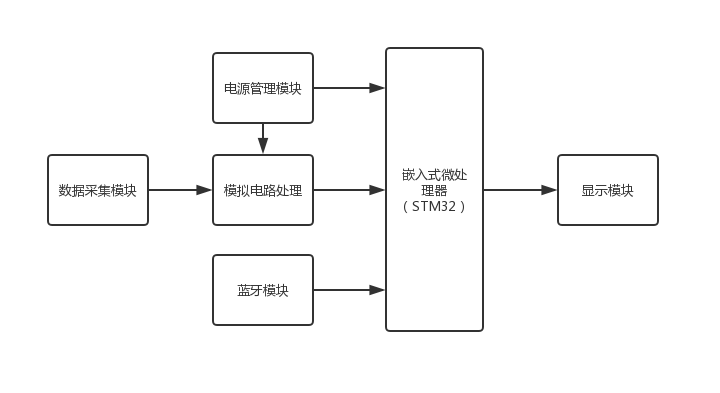
\includegraphics[scale = 0.58 ]{1-1.png}
    \caption{设计总体框图}
    \label{img1} 
  \end{figure}
\par{} 由上图可知,我们通过传感器进行数据采集,进一步进行模拟电路对数据处理,再通过模数转换电路驱动单片机,除此之外由电源管理模块为单片机以及模拟部分提供稳压电源,并另行有蓝牙模块与手机进行通讯,而数字部分的处理全部交由STM32完成,最终进行显示。

\subsubsection{结果反馈方法}
\par{} 我们计划使用LED或LCD显示屏将收集到的数据进行显示,显示内容包括以上叙述的测量指标,时间日期等,并加入阈值报警,若超过规定的阈值,则通过蜂鸣器进行报警。其次利用蓝牙模块与手机进行连接,将测量结果可以在用户手机上进行实时的显示,能够极其方便的获取当前环境情况。

\section{方案比较与选择}\label{sect1}
\par{} 通过我们对文献的查阅以及阅读,可以看到大多数基于单片机的大气环境检测系统,都是选择一款合适的单片机或其他微处理器作为主控,也即系统的核心,通过各个传感器与主控的连接进行数据的处理,最后通过LCD显示屏来进行结果的反馈。在整体上这些方案大同小异,但为我们的设计提供了思路与基础,而方案的选择也体现在细节方面的主控芯片的选择以及传感器的选择。
\subsection{文献方案叙述}
\par{} 首先叙述总结在文献中获得的方案设计,为了比较不同,我选择了其中的一篇基于ARM的多功能环境检测系统与基于STC90C51单片机的多功能检测系统分别进行介绍。
\subsubsection{基于ARM的多功能环境检测系统}
\par{} 首先我查阅到ARM处理器是英国Acorn有限公司设计的低功耗成本的第一款RISC微处理器。具有体积小、低功耗、低成本、高性能等优势。而在文章\footnote{引用文章,见于参考文献1中}的设计中以ARM作为主控单元,还包括PM2.5传感器单元、温湿度传感器单元、液晶显示屏单元、语音实时播报单元、外部事件触发单元\cite{曲爱玲2017基于}。整体可以由如下的框图实现:
\begin{figure}[H]
  \centering
  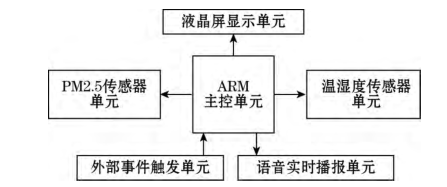
\includegraphics[scale = 0.7 ]{1-2.png}
  \caption{ARM设计总体框图}
  \label{img2} 
\end{figure}
\par{} 主控单元与模块化的思路是对于类似系统设计的基本思路,也是我们阅读的文献的共同思路,而其他传感单元由于可替换性因此需要我们加以选择。
\par{} 首先主控单元采用了ARM,可使用KEIL4编译软件环境进行开发,同时可利用C语言进行程序的编写,开发时十分方便快捷。
\par{} PM2.5浓度传感器其采用PMS70XX系列超薄数字式通用颗粒物浓度传感器。经查阅其中文手册,得知该传感器工作原理图如下所示:
\begin{figure}[H]
  \centering
  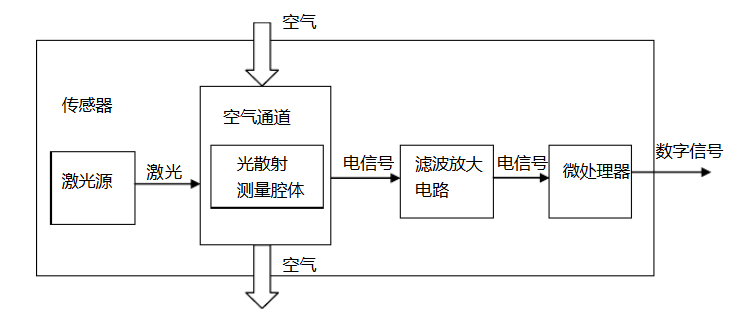
\includegraphics[scale = 0.65 ]{1-3.png}
  \caption{PM570XX系列传感器}
  \label{img3} 
\end{figure}
\par{} 其主要通过激光源发射激光经过腔体,在腔体内由于颗粒物浓度不同导致散射光强不同,进而能够转化为电信号,从而利用反射光强来反馈出细微颗粒物的浓度,直流供电电压为5V,最大工作电流为100mA,工作温度范围为$-20^{\circ} C\sim 50^{\circ}C$,传输协议为默认波特率9600Kbps,无校验位,有一位停止位。
\par{} 液晶显示屏采用一个3.5英寸的TFT LCD液晶屏,320$\times 240$像素,26万色,支持触摸屏功能,能够较好的进行显示。其他单元模块芯片不再赘述。
\subsubsection{基于STC90C51的检测系统}
\par{} 该检测系统为我所阅读文献中另一篇较具有代表性的文献,其设计除主控单元不同外,在传感器的选取上也与上一个单元有所不同,因此特此拿来与上一个系统进行比较分析,同样首先从整体框图上说明该系统的工作原理。
\begin{figure}[H]
  \centering
  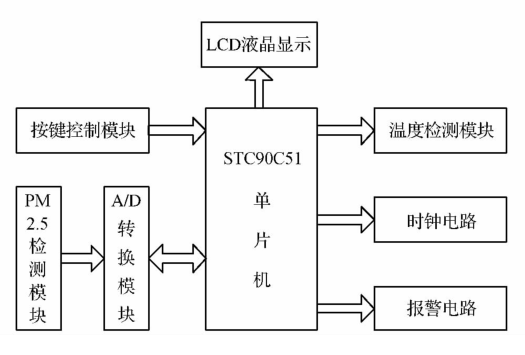
\includegraphics[scale = 0.65 ]{1-4.png}
  \caption{STC90C51总体框图}
  \label{img4} 
\end{figure}

\par{} 可见该系统总体框图与ARM系统基本相似,均以单片机作为主控单元,各模块电路通过硬件连接与主控单元进行相连与交互,只是该系统的设计中外接部分单元电路的功能不同。
\par{} 其主控单元为STC90C51单片机,为一款高速低功耗单片机,其在编译环境以及编程的方便性与可移植性等方面与其他单片机并无较大差别,因此也非选择的重点。
\par{} 其PM2.5检测模块使用的传感器为GP2Y1050AU0F灰尘传感器,是夏普公司开发的二代PM2. 5传感器\cite{陈卓2016一种},输出电压在$0\sim 3.5V$的范围内,电流损耗最大为20mA。在无尘时输出电压为0V,其原理如下图[\ref{img5}]所示:
\begin{figure}[H]
  \centering
  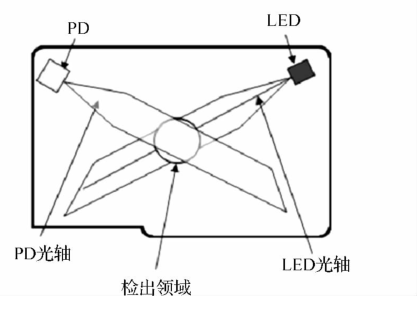
\includegraphics[scale = 0.65 ]{1-5.png}
  \caption{GP2Y1050AU0F灰尘传感器结构}
  \label{img5} 
\end{figure}
\par{} 检测原理为灰尘或烟雾颗粒通过防尘通气孔进入装置,红外发光二极管发射红外线到颗粒物上,光敏三极管接收其散射光信号。可见其原理与PM570XX系列相似,第二代PM2. 5传感器能随使用时间的增长自动计算和优化损耗\cite,能够在较长时间的使用后保证输出数据的准确性,相对而言体现了此传感器的优势。
\par{} 在此设计中采用ADS7822进行模数转换,其输入与传感器的模拟输出相连,作用是将传感器输出的模拟电压信号经过 A/D 转换,再由单片机数据采集、计算、处理。ADS7822是TI公司的低功耗,高性能12位A/D转换芯片,正常模式下典型功耗为0.54mW。
\par{} 其使用的温度模块采用了DS18B20数字温度传感器,其具9 Bit至12Bit的摄氏温度测量精度,测量范围为-55$\sim +125^{\circ}C$,可以直接由数据线进行供电而不需要外部电源,因此可以外部电源的使用。
\par{} 综上所述介绍的两种具有多功能的PM2.5检测仪,为我们的设计提供了基本的思路与选择的方向,我们旨在设计出具有更多功能的环境舒适度测量仪,以上pm2.5的多功能模块的总体方案为我们的设计的重要部分,接下来我将继续介绍我们的整体方案选择。
\subsection{方案选择}
\par{} 综合考虑我们选用Arduino单片机作为主控模块,其余相应单元模块进行了芯片的初步选择,这既考虑到芯片供电电压的选取与我们电源管理电路模块尽量相符,又兼并考虑了芯片的精度,工作范围等条件,下面依次介绍我们所选取的芯片,电路框图类比于以上两种设计,我们的设计如下:
\begin{figure}[H]
  \centering
  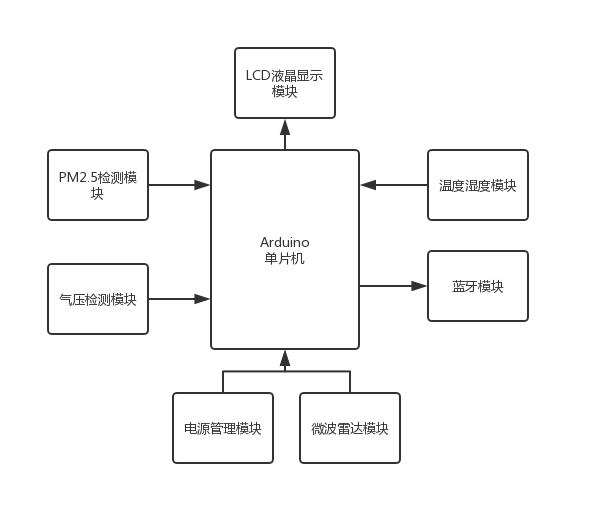
\includegraphics[scale = 0.45 ]{1-n.png}
  \caption{简略框图}
  \label{img6} 
\end{figure}
\subsubsection{单片机Arduino}

\subsubsection{GP2Y1050AU0F灰尘传感器}

\subsubsection{DHT-11温度湿度传感器}

\subsubsection{LCD1602液晶显示屏}

\subsubsection{TTP226电容触摸开关}


\section{基于WEBENCH的电源电路仿真}
\section{电路框图}

\section{数字系统流程图}


\bibliographystyle{plain}
\bibliography{yuxi}
\end{document}